\documentclass[10pt,twocolumn]{article}
\usepackage[margin=0.72in,columnsep=0.24in]{geometry}
\usepackage{amsmath,amssymb,booktabs,graphicx,microtype,siunitx,xcolor,hyperref,enumitem,balance}
\hypersetup{colorlinks=true,linkcolor=blue!55!black,citecolor=blue!55!black,urlcolor=blue!55!black}
\setlist{nosep,leftmargin=*}
\sisetup{detect-all}
\graphicspath{{figures/}}
\newcommand{\TotalRows}{5,400}
\newcommand{\CompleteRows}{5,372}
\newcommand{\FailedRows}{28}
\newcommand{\ReadoutFailures}{28}
\newcommand{\ReadoutFailureRate}{1.56\%}
\newcommand{\CompleteOperatingCells}{34}
\newcommand{\RawWins}{9}
\newcommand{\ReadoutWins}{21}
\newcommand{\ZNEWins}{4}
\newcommand{\ZNEOutOfRange}{5}
\newcommand{\RawRMSE}{0.2793}
\newcommand{\RawBias}{-0.1910}
\newcommand{\ReadoutRMSE}{0.1647}
\newcommand{\ReadoutBias}{-0.1047}
\newcommand{\ZNERMSE}{0.2415}
\newcommand{\ZNEBias}{-0.1566}

\title{Adaptive Quantum Error Mitigation Under Fixed Shot Budgets:\\
A Reproducible Simulator Benchmark}
\author{Zhen-Jun Liu}
\date{November 2, 2026}
\begin{document}
\maketitle
\begin{abstract}
Quantum error mitigation (QEM) can reduce bias without encoding a logical qubit, but
its auxiliary executions and statistical amplification consume finite sampling
resources. This study asks when unmitigated estimation, full-assignment-matrix
readout mitigation, and linear zero-noise extrapolation (ZNE) are useful under the
same total shot budget. We evaluate $X^{\otimes w}$ on simulated GHZ circuits with
widths $w\in\{2,4,6\}$, four idealized mixed-noise levels, three shot budgets, and 50
deterministic repeats per applicable operating cell. Among 34 cells for which all
three methods completed 50 repeats, readout mitigation attained the lowest
root-mean-square error (RMSE) in \ReadoutWins{} cells, raw estimation in \RawWins{},
and linear ZNE in \ZNEWins{}. Across completed rows, the respective RMSE values were
\ReadoutRMSE{}, \RawRMSE{}, and \ZNERMSE{} for readout, raw, and ZNE. Readout
mitigation also failed explicitly in \FailedRows{} width-6, 1,024-shot rows because
the sampled calibration matrix was ill-conditioned. The evidence is entirely
analytic or simulated; it does not establish performance on quantum hardware or
under calibrated device noise.
\end{abstract}
\section{Introduction}
Near-term quantum computations often estimate expectation values from noisy,
finite-shot measurements. QEM methods seek to reduce the resulting error without
the qubit overhead of full error correction, but they introduce sampling and
classical-processing overhead and can amplify variance
\cite{temme2017,li2017,cai2023}. Consequently, applying mitigation is not a
method-independent prescription: effectiveness depends on the circuit, observable,
noise channel, and resource budget.

The research question is: \emph{under a fixed total shot budget, which of raw
estimation, readout mitigation, and linear ZNE minimizes estimation error, and where
does mitigation fail or waste resources?} The repository implements a simulator-only
benchmark with deterministic seeds, repeat-level raw data, explicit resource
accounting, and failure statuses. The contribution is an auditable operating-regime
comparison, not a claim of new QEM theory or hardware advantage.
\section{Methodology}
\subsection{Reference state and observable}
For width $w$, the benchmark prepares
\begin{equation}
  \lvert \mathrm{GHZ}_w\rangle =
  \frac{\lvert 0\rangle^{\otimes w}+\lvert 1\rangle^{\otimes w}}{\sqrt{2}},
  \label{eq:ghz}
\end{equation}
using one Hadamard gate followed by $w-1$ controlled-NOT gates. The primary
observable is $P_w=X^{\otimes w}$, for which the analytic prediction and noiseless
statevector result are
\begin{equation}
  \mu_{\mathrm{ref}}=\langle \mathrm{GHZ}_w\rvert P_w
  \lvert \mathrm{GHZ}_w\rangle=1.
  \label{eq:reference}
\end{equation}
Tests cross-check this relation to absolute tolerance $10^{-12}$ for
$w\in\{2,4,6\}$.

For $N$ shots with parity eigenvalues $y_s\in\{-1,+1\}$, the raw estimator and
plug-in shot-noise standard error are
\begin{align}
  \widehat{\mu} &= \frac{1}{N}\sum_{s=1}^{N}y_s,\label{eq:estimator}\\
  \widehat{\sigma}_{\widehat{\mu}} &=
  \sqrt{\frac{1-\widehat{\mu}^{\,2}}{N}}.\label{eq:se}
\end{align}
\subsection{Noise model}
Qiskit Aer supplies the noisy target-circuit simulation \cite{qiskitaer}. The
diagnostic mixed-noise model combines independent assignment error, one-qubit
depolarizing error, and two-qubit depolarizing error. Table~\ref{tab:noise} records
the exact simulator parameters. These values are controlled study factors, not
device calibrations.
\begin{table}[t]
\centering
\caption{The four simulated noise levels increase readout and depolarizing error
together; none is assigned to a physical device.}
\label{tab:noise}
\begin{tabular}{lrrrr}
\toprule
Level & $p_{01}$ & $p_{10}$ & $p_{1q}$ & $p_{2q}$\\
\midrule
Zero & 0 & 0 & 0 & 0\\
Low & .005 & .004 & .001 & .010\\
Medium & .020 & .016 & .005 & .030\\
High & .050 & .040 & .010 & .080\\
\bottomrule
\end{tabular}
\end{table}
\subsection{Readout mitigation}
For width $w$, all $2^w$ computational basis states are calibrated. If
$A_{ij}=\Pr(\mathrm{observe}\ i\mid\mathrm{prepare}\ j)$ and
$\widehat{\boldsymbol p}_{\mathrm{obs}}$ is the observed probability vector, the
corrected distribution solves
\begin{equation}
  \widehat{\boldsymbol p}=\underset{\boldsymbol p\geq 0}{\arg\min}
  \lVert A\boldsymbol p-\widehat{\boldsymbol p}_{\mathrm{obs}}\rVert_2,
  \quad \mathbf{1}^{\mathsf T}\widehat{\boldsymbol p}=1.
  \label{eq:readout}
\end{equation}
This constrained correction follows the assignment-matrix approach
\cite{bravyi2021}. A condition number above $10^8$ or a non-finite value produces an
explicit \texttt{ill\_conditioned} status. The total budget is split
deterministically: 20\% for calibration and 80\% for the target. Calibration
observations are sampled directly from the declared independent assignment channel
with seeded multinomial draws; no hardware calibration data are used.
\subsection{Linear zero-noise extrapolation}
Global unitary folding constructs
\begin{equation}
  U_{\lambda}=U(U^{\dagger}U)^{(\lambda-1)/2},
  \quad \lambda\in\{1,3,5\},
  \label{eq:folding}
\end{equation}
which is ideally equivalent to $U$ while increasing noisy gate exposure. This is a
standard digital noise-scaling mechanism \cite{giurgica2020}. The fixed total shot
budget is divided across the three factors. Before the full benchmark, the analysis
model was fixed as ordinary least squares,
\begin{equation}
  \widehat{\mu}(\lambda)=\beta_0+\beta_1\lambda,
  \qquad \widehat{\mu}_{\mathrm{ZNE}}=\beta_0.
  \label{eq:zne}
\end{equation}
Extrapolates are retained without clipping and flagged when outside $[-1,1]$.
\subsection{Metrics}
For completed repeats $r=1,\ldots,R$, let
$e_r=\widehat{\mu}_r-\mu_{\mathrm{ref}}$. The reported metrics are
\begin{align}
  \mathrm{bias} &= R^{-1}\sum_r e_r,\\
  \mathrm{variance} &= (R-1)^{-1}\sum_r
  (\widehat{\mu}_r-\overline{\mu})^2,\\
  \mathrm{RMSE} &= \sqrt{R^{-1}\sum_r e_r^2}.
  \label{eq:metrics}
\end{align}
Method-level summaries are repeat-weighted and conditional on completion. The
operating-regime winner is defined only where all three methods have 50 completed
repeats, avoiding comparison against a partially failed method.
\section{Experiment Setup}
The frozen manifest crosses widths $2,4,6$; declared depths $1,3,6$; four noise
levels; shot budgets $1{,}024$, $4{,}096$, and $16{,}384$; three methods; and 50
repeat seeds. GHZ preparation is defined only at depth parameter 1, so depths 3 and
6 remain in the manifest as \texttt{not\_applicable}. The applicable benchmark
contains \TotalRows{} repeat-level rows across 36 operating cells and three methods.

All stochastic seeds derive from root seed 20261102 through SHA-256 namespacing.
Raw estimation spends all shots on the target. Readout mitigation charges every
calibration shot to the same total budget. ZNE charges all three folded-circuit
executions to that budget. The environment is Python 3.12 with Qiskit 2.2.3, Qiskit
Aer 0.17.2, NumPy 2.3.4, SciPy 1.16.3, and pandas 2.3.3.

Figure~\ref{fig:folding} verifies that folding increases transpiled depth while tests
establish ideal-unitary equivalence to $10^{-12}$.
\begin{figure}[t]
\centering
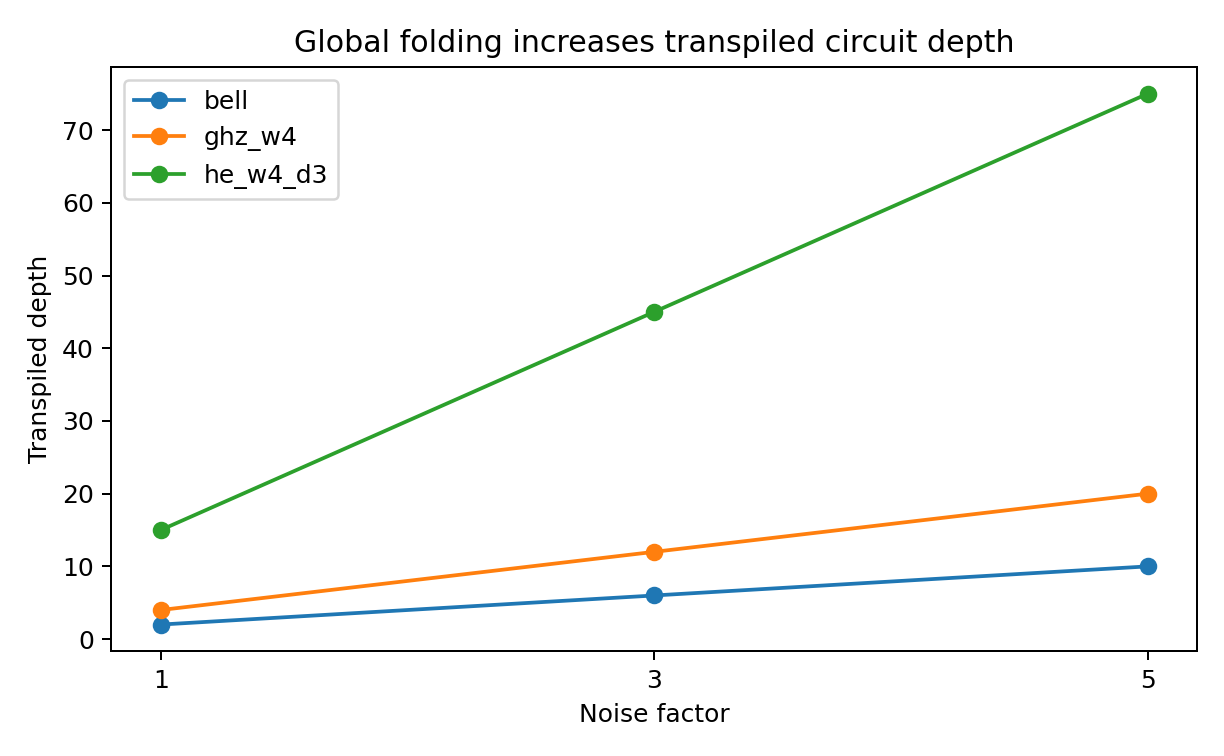
\includegraphics[width=\columnwidth]{day08_depth_vs_noise_factor.png}
\caption{Global folding increases transpiled depth for the tested Bell, GHZ, and
hardware-efficient circuits while preserving the ideal unitary in tests.}
\label{fig:folding}
\end{figure}
\section{Results}
\subsection{Aggregate error and operating regimes}
Figure~\ref{fig:rmse} shows completed-row RMSE by simulated noise. Zero-noise results
agree with the analytic reference up to floating-point precision. Beyond zero noise,
readout mitigation has the lowest aggregate RMSE: \ReadoutRMSE{} overall, compared
with \ZNERMSE{} for linear ZNE and \RawRMSE{} for raw estimation. These aggregates
do not mean that readout wins every condition.
\begin{figure}[t]
\centering
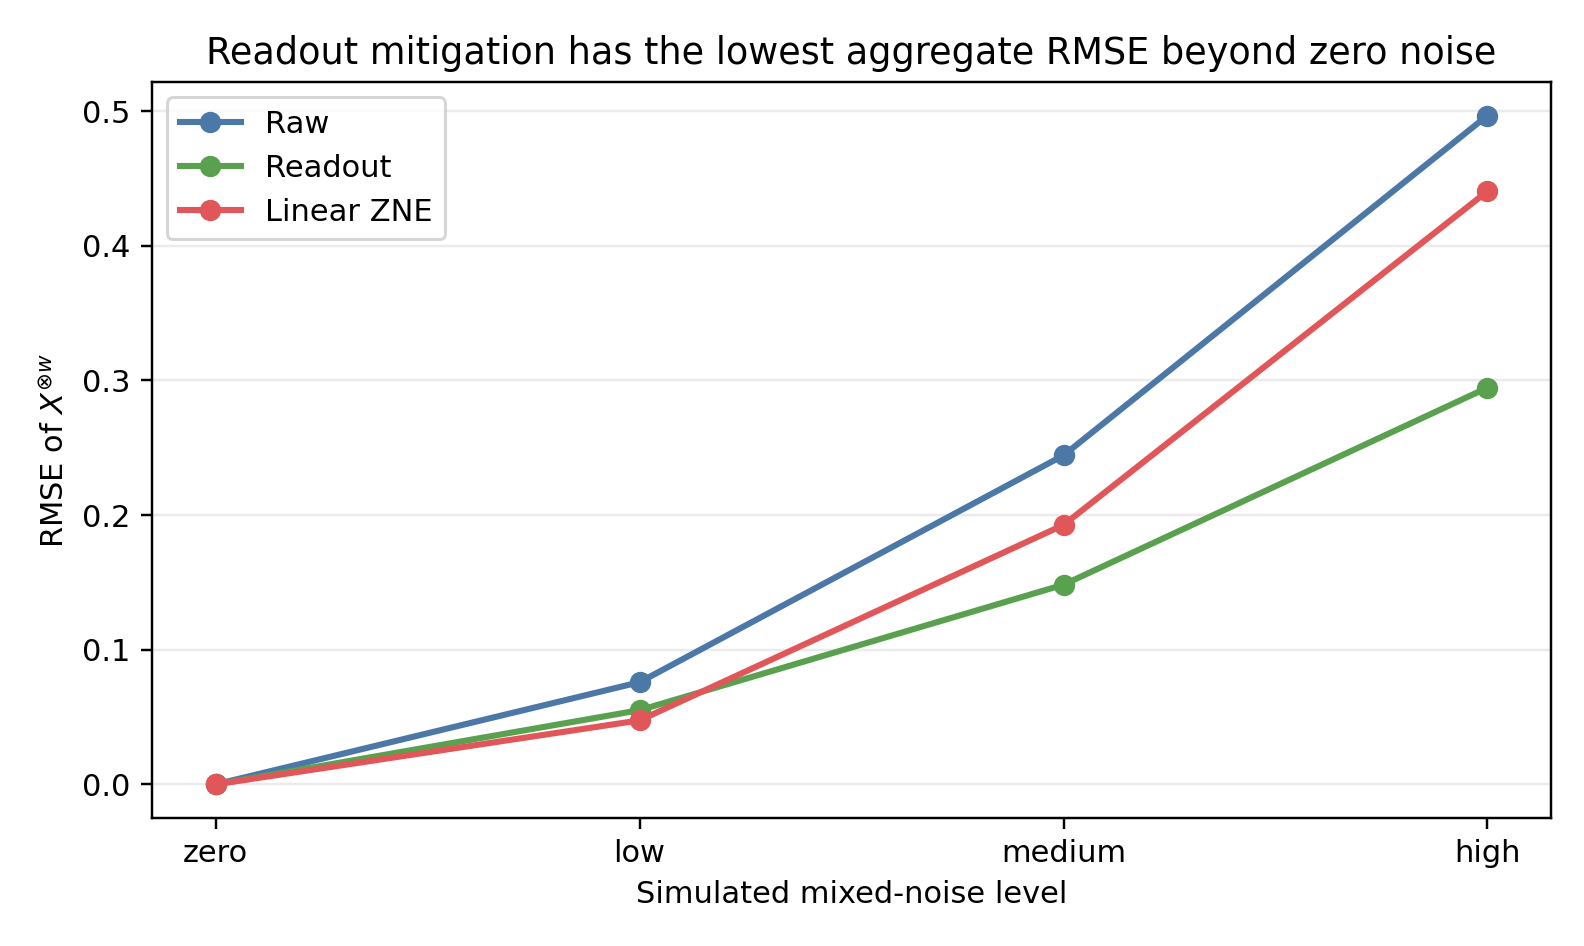
\includegraphics[width=\columnwidth]{rmse_by_noise.png}
\caption{Across completed simulated rows, readout mitigation has lower RMSE than raw
estimation and linear ZNE at low, medium, and high mixed-noise levels.}
\label{fig:rmse}
\end{figure}
\begin{table*}[t]
\centering
\caption{Completed-row bias and RMSE depend on method and simulated noise. Readout
has fewer completed rows at medium and high noise because failed rows have no numeric
estimate.}
\label{tab:noise-results}
\begin{tabular}{llrrr}
\toprule
Noise & Method & Completed & Bias & RMSE\\
\midrule
Zero & Raw & 450 & 0.0000 & 0.0000 \\
Zero & Readout & 450 & 0.0000 & 0.0000 \\
Zero & Linear ZNE & 450 & 0.0000 & 0.0000 \\
Low & Raw & 450 & -0.0685 & 0.0759 \\
Low & Readout & 450 & -0.0465 & 0.0551 \\
Low & Linear ZNE & 450 & -0.0416 & 0.0475 \\
Medium & Raw & 450 & -0.2261 & 0.2443 \\
Medium & Readout & 447 & -0.1246 & 0.1483 \\
Medium & Linear ZNE & 450 & -0.1757 & 0.1927 \\
High & Raw & 450 & -0.4695 & 0.4967 \\
High & Readout & 425 & -0.2563 & 0.2946 \\
High & Linear ZNE & 450 & -0.4091 & 0.4405 \\
\bottomrule

\end{tabular}
\end{table*}

Figure~\ref{fig:regimes} resolves the aggregate into 36 width--noise--budget
conditions. Of the \CompleteOperatingCells{} fully completed cells, readout has the
lowest RMSE in \ReadoutWins{}, raw estimation in \RawWins{}, and linear ZNE in
\ZNEWins{}. No method dominates the complete operating grid.
\begin{figure*}[t]
\centering
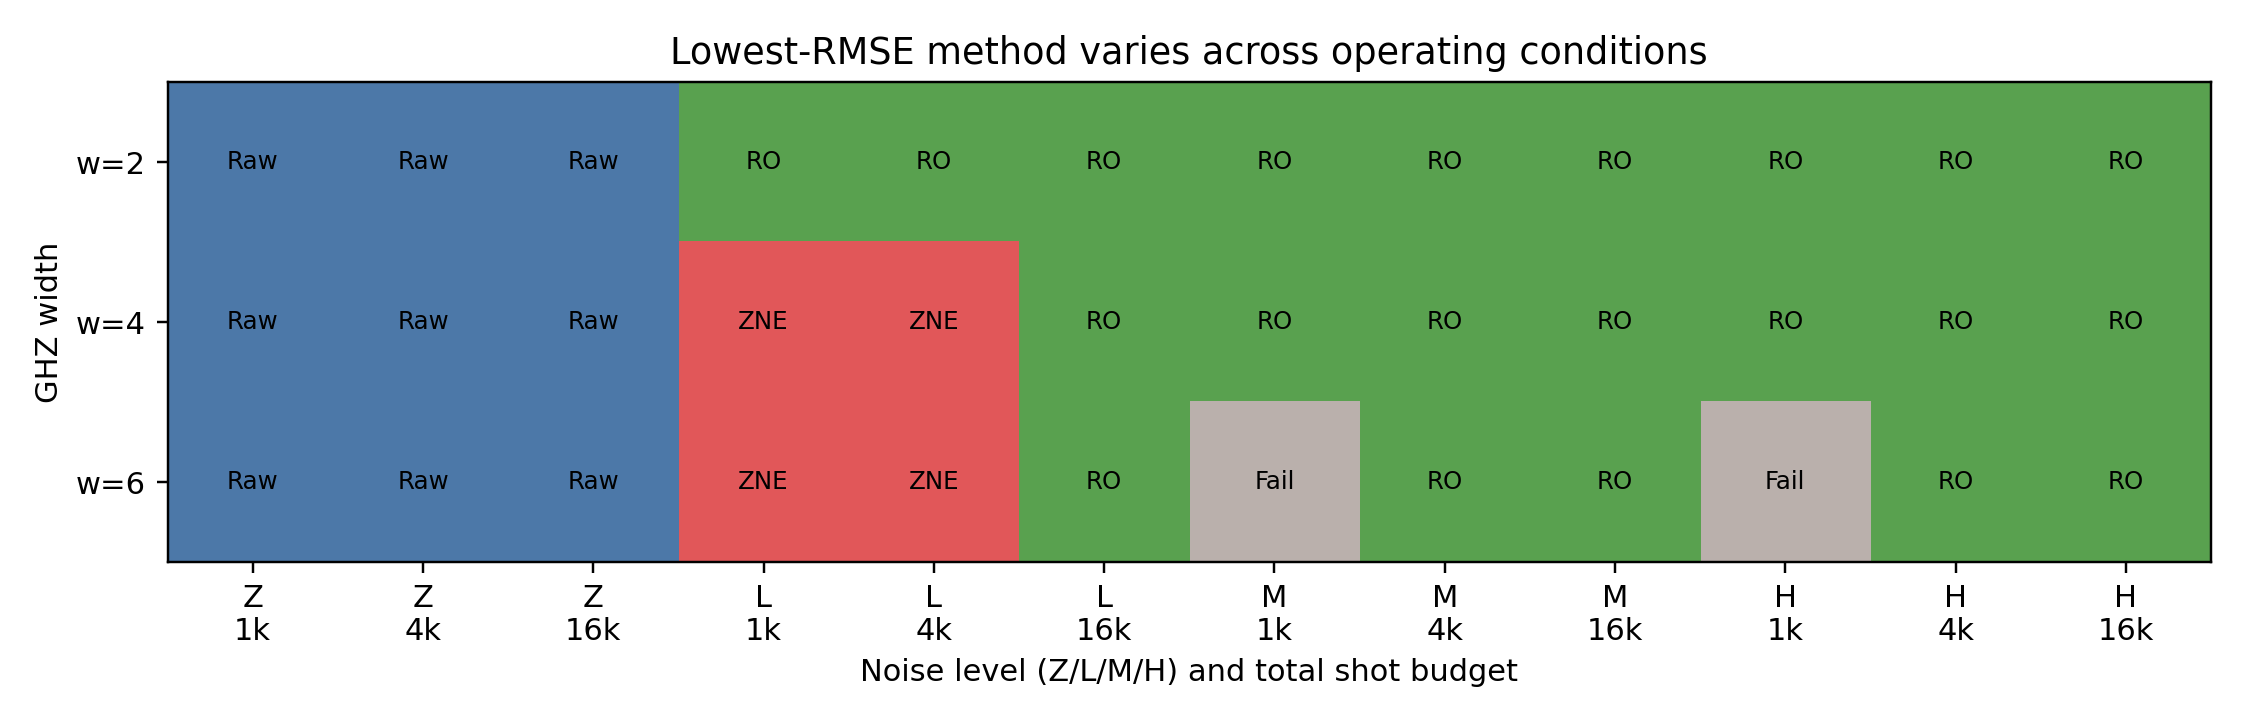
\includegraphics[width=0.93\textwidth]{operating_regime_map.png}
\caption{The minimum-RMSE method changes with width, noise, and total shots.
Failed conditions are excluded because readout did not complete all 50 repeats.}
\label{fig:regimes}
\end{figure*}
\subsection{Explicit readout failures}
The run retains \CompleteRows{} completed and \FailedRows{} failed rows. All failures
occur for width 6, total budget 1,024, and readout mitigation
(Table~\ref{tab:failures}). They represent \ReadoutFailureRate{} of the 1,800
readout rows. With 20\% calibration allocation, 204 shots are divided among 64 basis
states, leaving three or four samples per calibration column; the sampled assignment
matrix can be singular or exceed the condition-number threshold. This is a supported
numerical diagnosis; its hardware relevance remains untested.
\begin{table}[t]
\centering
\caption{All failed simulated rows are explicit conditioning failures at the
smallest budget and largest width.}
\label{tab:failures}
\resizebox{\columnwidth}{!}{%
\begin{tabular}{rrrrrl}
\toprule
$w$ & Noise & Shots & Method & Count & Status\\
\midrule
6 & High & 1,024 & Readout & 25 & Ill-conditioned assignment matrix \\
6 & Medium & 1,024 & Readout & 3 & Ill-conditioned assignment matrix \\
\bottomrule

\end{tabular}}
\end{table}
\subsection{ZNE behavior}
The preregistered three-factor linear fit improves aggregate RMSE over raw estimation
but wins only \ZNEWins{} complete cells. Only \ZNEOutOfRange{} nontrivial
extrapolates exceed the Pauli range by more than $10^{-12}$; they remain unclipped.
Figure~\ref{fig:zne} shows factor estimates and the fit for the first Day 9 validation
repeat. It illustrates the estimator, not the full performance distribution.
\begin{figure}[t]
\centering
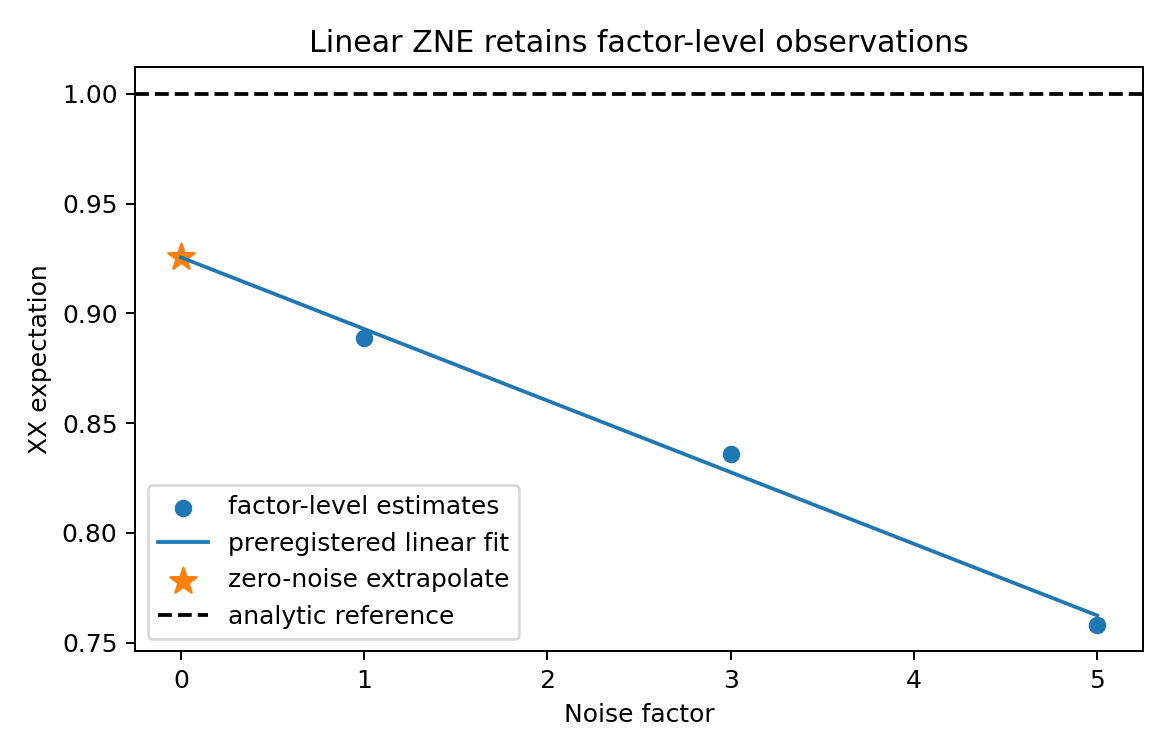
\includegraphics[width=\columnwidth]{day09_zne_extrapolation_lambda-1-3-5.png}
\caption{The validation artifact preserves all three noisy estimates and the
preregistered extrapolate instead of reporting only a corrected value.}
\label{fig:zne}
\end{figure}
\section{Conclusion}
Under the declared simulator model and equal total shot budgets, QEM effectiveness is
operating-regime dependent. Readout mitigation produced the lowest RMSE most often
and the lowest aggregate RMSE, but failed when full-matrix calibration was
undersampled. Linear ZNE improved aggregate RMSE relative to raw estimation yet was
best in only a minority of complete cells. The evidence supports a selector based on
width, noise, budget, and method status; it does not support unconditional mitigation.
\section{Discussion}
\subsection{Evidence-supported findings}
The comparison demonstrates that mitigation overhead must be charged explicitly,
aggregate performance hides regime changes, and failure status is part of method
performance. Raw estimation remains preferable in \RawWins{} fully completed cells.
Omitting the 28 ill-conditioned rows would overstate readout reliability.
\subsection{Interpretation and hypotheses}
Readout mitigation likely performs well because its calibration uses the same
independent assignment channel applied to target measurements. This is an
interpretation, not evidence that it remains best under correlated readout, drift, or
device calibration error. Linear ZNE may underperform because a first-order model is
restrictive and the fixed budget leaves about one third of the shots at each factor.
The benchmark does not isolate these possible causes.
\subsection{Limitations}
All noisy results are Qiskit Aer simulations with idealized, stationary, Markovian
channels. The study contains no hardware-derived or physical experimental data and
models no crosstalk, leakage, relaxation, drift, compilation variability, or coherent
calibration error. The GHZ benchmark uses only $X^{\otimes w}$ and widths up to six;
the declared depth sweep is not applicable. Full-matrix calibration scales as
$2^w$. Method-level RMSE is conditional on completion, and the operating map
contains only 34 complete comparisons. The fixed seed set is not a confidence
statement about real devices. No learned or optimized selector is evaluated.
\appendix
\section{Reproducibility and Data Contract}
\begin{verbatim}
python -m pytest
python -m src.generate_artifacts
python -m src.generate_days08_12
python -m src.generate_paper_assets
tectonic paper/main.tex --outdir paper
\end{verbatim}
Repeat-level observations remain under \texttt{results/raw/}; processed coverage is
separate. Seeds, statuses, count payloads, and method diagnostics are retained.
Wall-clock measurements are excluded from scientific raw rows because they are
nondeterministic and are reported separately.
\section{Analytic and Test Controls}
Tests check q0-first bit ordering, seed derivation, Bell and GHZ analytic expectations,
statevector agreement, folding equivalence, exact shot accounting, calibration
identity, explicit ill-conditioning, ZNE factors, manifest completeness, and
deterministic row execution. These validate implementation invariants, not physical
fidelity of the noise model.
\balance
\bibliographystyle{abbrv}
\bibliography{references}
\end{document}
